% ------------------------------------------------------------------------------
% TYPO3 Version 10.0 - What's New (English Version)
%
% @author	Michael Schams <schams.net>
% @license	Creative Commons BY-NC-SA 3.0
% @link		http://typo3.org/download/release-notes/whats-new/
% @language	English
% ------------------------------------------------------------------------------

\section{Modifiche per sviluppatori}
\begin{frame}[fragile]
	\frametitle{Modifiche per sviluppatori}

	\begin{center}\huge{Capitolo 4:}\end{center}
	\begin{center}\huge{\color{typo3darkgrey}\textbf{Modifiche per sviluppatori}}\end{center}

\end{frame}

% ------------------------------------------------------------------------------
% TYPO3 Version 10.0 - Breaking Changes

\begin{frame}[fragile]
	\frametitle{Changes for Integrators}
	\framesubtitle{Modifiche importanti}

	\small
		Informazione per gli sviluppatori: in TYPO3 v9, parti di codice PHP, TSconfig, TypoScript
            opzioni e condizioni, nonché la pianificazione dello scheduler sono stati segnati come deprecati.

		\vspace{0.2cm}

		In conformità alla \textbf{deprecation policy} di TYPO3, questi componenti sono stati
		rimossi in TYPO3 v10.0.

		\vspace{0.2cm}

		Questo include anche alcuni hook, annotazioni PHP (come ad esempio \texttt{@inject} e
		\texttt{@validate}), e alcuni cambiamenti di visibilità (es. da
		"\texttt{public}" a "\texttt{protected}").

		\vspace{0.2cm}

		Abilitate il deprecation log, verificate attentamente il vostro codice ed esaminate i log per
		individuare possibili problemi. Usate l'
		\href{https://docs.typo3.org/m/typo3/reference-coreapi/master/en-us/ApiOverview/ExtensionScanner/Index.html}{Extension Scanner}
		integrato per ottenere un rapporto completo delle incompatibilità delle estensioni.

	\normalsize

\end{frame}

% ------------------------------------------------------------------------------
% Feature | 88643 | New Mail API based on symfony/mailer and symfony/mime
% Breaking | 88643 | Removed Swiftmailerswiftmailer Dependency

\begin{frame}[fragile]
	\frametitle{Changes for Developers}
	\framesubtitle{Nuove Mail API}

	\begin{itemize}
		\item SwiftMailer è stato sostituito da librerie più moderne:

			\begin{itemize}
				\item \texttt{symfony/mime} per creare messaggi di tipo email
				\item \texttt{symfony/mailer} per inviare le email
			\end{itemize}

		\item La funzione PHP \texttt{mail()} non è più supportata.

			\begin{itemize}\smaller
				\item[\ding{228}] Si consiglia di passare a \texttt{sendmail} o \texttt{smtp} in alternativa.
			\end{itemize}\normalsize

		\item Plugin personalizzati con SwiftMailer e il suo utilizzo devono essere migrati.

		\item Vedi la \href{https://symfony.com/doc/current/mailer.html}{documentazione Symfony}
			per maggiori dettagli su come sfruttare le nuove funzionalità delle Mail API.
	\end{itemize}

\end{frame}

% ------------------------------------------------------------------------------
% Feature | 84112 | Symfony dependency injection for core and Extbase

\begin{frame}[fragile]
	\frametitle{Changes for Developers}
	\framesubtitle{Symfony Dependency Management/Injection (1)}

	\begin{itemize}
		\item Il pacchetto \texttt{symfony/dependency-injection} è stato integrato
			ed è utilizzato per gestire la gestione delle dipendenze a livello di sistema e l'injection
			di dipendenze nelle classi.

		\item Questo approcio mira a sostituire il gestore di injection di Extbase
			e il gestore degli oggetti.

		\item Pertanto, le seguenti classi dovrebbero essere adattate ed evitate (quando possibile):

			\begin{itemize}\small
				\item \texttt{\textbackslash
					TYPO3\textbackslash
					CMS\textbackslash
					Extbase\textbackslash
					Object\textbackslash
					ObjectManager}
				\item \texttt{\textbackslash
					TYPO3\textbackslash
					CMS\textbackslash
					Core\textbackslash
					Utility\textbackslash
					GeneralUtility::makeInstance()}
			\end{itemize}\normalsize

	\end{itemize}

\end{frame}

% ------------------------------------------------------------------------------
% Feature | 84112 | Symfony dependency injection for core and Extbase

\begin{frame}[fragile]
	\frametitle{Changes for Developers}
	\framesubtitle{Symfony Dependency Management/Injection (2)}

	% decrease font size for code listing
	\lstset{basicstyle=\tiny\ttfamily}

	\begin{itemize}
		\item Le opzioni di configurazione includono:

			\begin{itemize}
				\item Autowiring (vedi esempio sotto)
				\item Manual wiring
					(vedi \href{https://docs.typo3.org/c/typo3/cms-core/master/en-us/Changelog/10.0/Feature-84112-SymfonyDependencyInjectionForCoreAndExtbase.html}{change log})
				\item Advanced functionality
					(vedi \href{https://docs.typo3.org/c/typo3/cms-core/master/en-us/Changelog/10.0/Feature-84112-SymfonyDependencyInjectionForCoreAndExtbase.html}{change log})
			\end{itemize}

		% \smaller Un esempio "autowiring":\normalsize

\begin{lstlisting}
# Configuration/Services.yaml
services:
  _defaults:
    autowire: true
    autoconfigure: true
    public: false

  Your\Namespace\:
    resource: '../Classes/*'
\end{lstlisting}

		\item Vedi la \href{https://symfony.com/doc/current/service_container.html}{documentazione Symfony} per maggiori dettagli.

	\end{itemize}

\end{frame}

% ------------------------------------------------------------------------------
% Feature | 88769 | Introduce a generic EventDispatcher based on PSR-14
% Feature | 88770 | Add PSR-14 EventDispatcher logic based on DI

\begin{frame}[fragile]
	\frametitle{Changes for Developers}
	\framesubtitle{Event Dispatching (1)}

	\begin{itemize}
		\item Un nuovo sistema di "EventDispatcher" è stato aggiunto e mira a sostituire
		    i concetti di Hook e Signal/Slots.

		\item E' basato sullo \href{https://www.php-fig.org/psr/psr-14}{standard PSR-14}
			che consente di fare injection in un'applicazione in modo facile e coerente.

		\item PSR-14 consiste nei 4 seguenti componenti:

			\begin{itemize}
				\item Un oggetto \textbf{EventDispatcher} che viene usato per attivare un evento.
				\item Un oggetto \textbf{ListenerProvider} che contiene registrati tutti gli "ascolti" degli eventi.
				\item Uno o più oggetti \textbf{Event} che sono chiamati dal core di TYPO3 o dalle estensioni ("Emitter").
				\item Uno o più \textbf{Listeners} (di solito in estensioni e pacchetti PHP) che sono registrati.
			\end{itemize}

% Short-Term goal is to deprecate SignalSlot dispatcher in TYPO3 v10,
% and migrate all signals to the EventDispatcher.

	\end{itemize}

\end{frame}

% ------------------------------------------------------------------------------
% Feature | 88769 | Introduce a generic EventDispatcher based on PSR-14
% Feature | 88770 | Add PSR-14 EventDispatcher logic based on DI

\begin{frame}[fragile]
	\frametitle{Changes for Developers}
	\framesubtitle{Event Dispatching (2)}

	% decrease font size for code listing
	\lstset{basicstyle=\tiny\ttfamily}

	Esempio di implementazione

	\begin{itemize}\smaller
		\item[\ding{202}] Aggiungi il tag \texttt{event.listener} nel file \texttt{Configuration/Services.yaml}:

\begin{lstlisting}
services:
  Vendor\Example\EventListener\NullMailer:
    tags:
      - { name: event.listener, identifier: 'myListener', event: TYPO3\CMS\Core\Mail\Event\AfterMailerInitializationEvent, before: 'redirects, anotherIdentifier' }
\end{lstlisting}

		\item[\ding{203}] Implementa il tuo oggetto evento:

\begin{lstlisting}
namespace Vendor\Example\EventListener;

class NullMailer
{
  public function __invoke(AfterMailerInitializationEvent $event): void
  {
    $event->getMailer()->injectMailSettings(['transport' => 'null']);
  }
}
\end{lstlisting}

	\end{itemize}\normalsize

\end{frame}

% ------------------------------------------------------------------------------
% Feature | 88769 | Introduce a generic EventDispatcher based on PSR-14
% Feature | 88770 | Add PSR-14 EventDispatcher logic based on DI

\begin{frame}[fragile]
	\frametitle{Changes for Developers}
	\framesubtitle{Event Dispatching (3)}

	% decrease font size for code listing
	\lstset{basicstyle=\tiny\ttfamily}

	\begin{itemize}
		\item La lista di tutti gli eventi Listeners disponibili è possibile vederla nel backend:\newline
			\smaller
				(necessita dell'estensione di sistema \texttt{EXT:lowlevel})
			\normalsize
	\end{itemize}

	\begin{figure}
		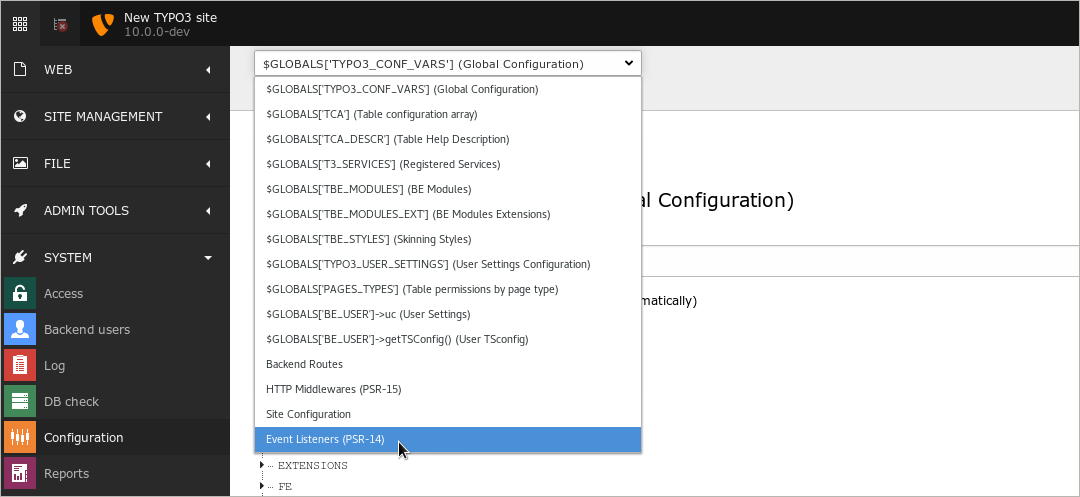
\includegraphics[width=0.70\linewidth]{ChangesForDevelopers/88770-PSR14-EventDispatcher.png}
	\end{figure}

\end{frame}


% ------------------------------------------------------------------------------
% Feature | 88769 | Introduce a generic EventDispatcher based on PSR-14
% Feature | 88770 | Add PSR-14 EventDispatcher logic based on DI

\begin{frame}[fragile]
	\frametitle{Changes for Developers}
	\framesubtitle{Event Dispatching (4)}

	% decrease font size for code listing
	\lstset{basicstyle=\tiny\ttfamily}

	\begin{itemize}
		\item Migliori pratiche:

			\begin{itemize}
				\item Aggiungi solo un Listener per classe PHP e usa \texttt{\_\_invoke()} come nome del metodo.
				\item Aggiungi il suffisso "\texttt{Event}" al nome della classe quando viene creata una nuova classe PHP Event.
				\item Sposta il file della classe PHP Event in una directory appropriata es. \texttt{Classes/Database/Event}.
				\item Usa l'injection di dipendenze sotto forma di argomento del costruttore per ricevere l'evento EventDispatcher,
				    se possibile.
			\end{itemize}

		\item Note aggiuntive:\newline
			\small
				Gli eventi forniti dal core di TYPO3 seguono la politica di deprecazione di TYPO3, ad eccezione dei suoi argomenti
				di costruzione che possono variare.
			\normalsize

	\end{itemize}

\end{frame}

% ------------------------------------------------------------------------------
% Feature | 88799 | Use PSR-3 interface for logging

\begin{frame}[fragile]
	\frametitle{Changes for Developers}
	\framesubtitle{Interfaccia PSR-3 Logger}

	\begin{itemize}
		\item Il Framework di Log di TYPO3 (in particolare LogLevel e LogManager) usano ora
			l'\href{https://www.php-fig.org/psr/psr-3/}{interfaccia PSR-3 Logger}.

		\item PSR-3 è un metodo standardizzato che permette alle librerie di ricevere un oggetto
			\texttt{Psr\textbackslash
				Log\textbackslash
				LoggerInterface} e di scrivere log in un modo semplice e universale.

			\item Questo permette agli sviluppatori di usare logger personalizzati e di interagire con altri sistemi
				di logging.

	\end{itemize}

\end{frame}

% ------------------------------------------------------------------------------
% Breaking | 88182 | jsfunc.inline.js has been dropped
% Breaking | 88427 | jsfunc.evalfield.js has been removed
% Breaking | 88667 | Removed additionalJavaScriptSubmit from FormEngine
% Deprecation | 88433 | Deprecate top.openUrlInWindow

\begin{frame}[fragile]
	\frametitle{Deprecated/Removed Functions}
	\framesubtitle{Funzioni e opzioni JavaScript (1)}

	\begin{itemize}
		\item I seguenti file JavaScript sono stati rimossi:

			\begin{itemize}
				\item \texttt{jsfunc.inline.js}
				\item \texttt{jsfunc.evalfield.js}
			\end{itemize}

			\begin{itemize}\smaller
				\item[\ding{228}] Usa \texttt{TYPO3/CMS/Backend/FormEngineValidation} in sostituzione.
			\end{itemize}\normalsize

		\item Prima era possibile inserire gestori di invio aggiuntivi tramite l'opzione \texttt{additionalJavaScriptSubmit}.
			Questa opzione è stata rimossa.

			\begin{itemize}\smaller
				\item[\ding{228}] Crea e registra un modulo AMD in alternativa.
			\end{itemize}\normalsize

		\item La funzione JavaScript globale \texttt{top.openUrlInWindow()} è stata segnata come deprecata.

	\end{itemize}

\end{frame}

% ------------------------------------------------------------------------------
% Breaking | 88411 | TBE_EDITOR.typo3form removed
% Deprecation | 88432 | Replaced md5js with an AMD module
% Deprecation | 88428 | top.rawurlencode and top.str_replace
% Deprecation | 88651 | Replace TYPO3/CMS/Backend/SplitButtons with TYPO3/CMS/Backend/DocumentSaveActions

\begin{frame}[fragile]
	\frametitle{Deprecated/Removed Functions}
	\framesubtitle{Funzioni e opzioni JavaScript (2)}

	\begin{itemize}

		\item L'oggetto globale \texttt{TBE\_EDITOR.typo3form} e i layer collegati \texttt{typo3FormFieldSet}
			e \texttt{typo3FormFieldGet} sono stati rimossi.

		\item Il file \texttt{md5.js} è stato segnato come deprecato.

			\begin{itemize}\smaller
				\item[\ding{228}] Carica il modulo AMD \texttt{TYPO3/CMS/Backend/Hashing/Md5} via RequireJS in alternativa.
			\end{itemize}\normalsize

		\item Le seguenti funzioni JavaScript globali sono state segnate come deprecate:

		\begin{itemize}
			\item \texttt{top.rawurlencode()}
			\item \texttt{top.str\_replace()}
		\end{itemize}

		\item Il modulo \texttt{TYPO3/CMS/Backend.SplitButtons} è diventato deprecato.

			\begin{itemize}\smaller
				\item[\ding{228}] Usa \texttt{TYPO3/CMS/Backend/DocumentSaveActions} in alternativa.
			\end{itemize}\normalsize

 	\end{itemize}

\end{frame}

% ------------------------------------------------------------------------------
% Important | 87894 | Removed PHP Dependency algo26-matthiasidna-convert

\begin{frame}[fragile]
	\frametitle{Changes for Developers}
	\framesubtitle{Domini UTF-8-based}

	\begin{itemize}
		\item PHP ha funzioni native per convertire i domini da UTF-8 al formato IDNA ASCII (“punicode”),
			per esempio \href{https://www.php.net/manual/en/function.idn-to-ascii.php}{idn\_to\_ascii()}.

		\item Queste possono essere usate direttamente se l'estensioni PHP
			"\href{https://www.php.net/manual/en/book.intl.php}{intl}" è installata.

		\item Se l'estensione PHP non è installata, il pacchetto \texttt{symfony/polyfill-intl-idn}
			fornisce ora le funzionalità.

		\item Precedentemente, era usato il pacchetto \texttt{algo26-matthias/idna-convert} che ora è stato rimosso.

	\end{itemize}

\end{frame}

% ------------------------------------------------------------------------------
% Feature | 87665 | Introduce BitSet class

\begin{frame}[fragile]
	\frametitle{Changes for Developers}
	\framesubtitle{Classe BitSet}

	% decrease font size for code listing
	\lstset{basicstyle=\tiny\ttfamily}

	\begin{itemize}
		\item Una nuova classe è stata introdotto per gestire in maniera efficiente le situazioni booleane:\newline
			\texttt{TYPO3\textbackslash
				CMS\textbackslash
				Core\textbackslash
				Type\textbackslash
				BitSet}

		\item Per esempio:

\begin{lstlisting}
define('PERMISSIONS_NONE', 0b0); // 0
define('PERMISSIONS_PAGE_SHOW', 0b1); // 1
define('PERMISSIONS_PAGE_EDIT', 0b10); // 2
define('PERMISSIONS_PAGE_DELETE', 0b100); // 4
define('PERMISSIONS_PAGE_NEW', 0b1000); // 8
define('PERMISSIONS_CONTENT_EDIT', 0b10000); // 16
define('PERMISSIONS_ALL', 0b11111); // 31

$bitSet = new \TYPO3\CMS\Core\Type\BitSet(PERMISSIONS_PAGE_SHOW | PERMISSIONS_PAGE_NEW);
$bitSet->get(PERMISSIONS_PAGE_SHOW); // true
$bitSet->get(PERMISSIONS_CONTENT_EDIT); // false
\end{lstlisting}

	\end{itemize}

\end{frame}

% ------------------------------------------------------------------------------
% Important | 87516 | Remove Core HTTP Request Handler Interface

\begin{frame}[fragile]
	\frametitle{Changes for Developers}
	\framesubtitle{Request Handler (1)}

	\begin{itemize}
		\item La seguente interfaccia interna è stata rimossa
			a favore delle interfacce di gestione e middleware di richiesta PSR-15:\newline
			\texttt{TYPO3\textbackslash
				CMS\textbackslash
				Core\textbackslash
				Http\textbackslash
				RequestHandlerInterface}

	\end{itemize}

\end{frame}

% ------------------------------------------------------------------------------
% Breaking | 88687 | Configure extbase request handlers via PHP

\begin{frame}[fragile]
	\frametitle{Changes for Developers}
	\framesubtitle{Request Handler (2)}

	% decrease font size for code listing
	\lstset{basicstyle=\tiny\ttfamily}

	\begin{itemize}
		\item La configurazione dei gestori di richieste Extbase non è più possibile con TypoScript

		\smaller\textbf{Vecchio} metodo in TypoScript:\normalsize
\begin{lstlisting}
config.tx_extbase {
  mvc {
    requestHandlers {
      Vendor\Example\Mvc\Web\FrontendRequestHandler = Vendor\Example\Mvc\Web\FrontendRequestHandler
    }
  }
}
\end{lstlisting}

		\smaller\textbf{Nuovo} metodo in file \texttt{Configuration/Extbase/RequestHandlers.php}:\normalsize
\begin{lstlisting}
<?php
declare(strict_types = 1);

return [
  \Vendor\Example\Mvc\Web\FrontendRequestHandler::class,
];
\end{lstlisting}

	\end{itemize}

\end{frame}


% ------------------------------------------------------------------------------
% Deprecation | 88366 | Default caching framework cache names changed

\begin{frame}[fragile]
	\frametitle{Changes for Developers}
	\framesubtitle{Caching Framework}

	% decrease font size for code listing
	\lstset{basicstyle=\tiny\ttfamily}

	\begin{itemize}
		\item Le seguenti cache sono state rinominate:

			\begin{itemize}\smaller
				\item \texttt{cache\_core} \textrightarrow\hspace{0.1cm}\texttt{core}
				\item \texttt{cache\_hash} \textrightarrow\hspace{0.1cm}\texttt{hash}
				\item \texttt{cache\_pages} \textrightarrow\hspace{0.1cm}\texttt{pages}
				\item \texttt{cache\_pagesection} \textrightarrow\hspace{0.1cm}\texttt{pagesection}
				\item \texttt{cache\_runtime} \textrightarrow\hspace{0.1cm}\texttt{runtime}
				\item \texttt{cache\_rootline} \textrightarrow\hspace{0.1cm}\texttt{rootline}
				\item \texttt{cache\_imagesizes} \textrightarrow\hspace{0.1cm}\texttt{imagesizes}
			\end{itemize}\normalsize

		\item Nuovi metodi per accedere alle cache:

\begin{lstlisting}
VECCHIO:
$cacheManager->getCache('cache_core').

NUOVO:
$cacheManager->getCache('core')
\end{lstlisting}

		\item Il prefisso \texttt{cf\_} è stato rimosso dalle tabelle del database.
	\end{itemize}

\end{frame}

% ------------------------------------------------------------------------------
% Deprecation | 87550 | Use controller classes when registering plugins/modules

\begin{frame}[fragile]
	\frametitle{Changes for Developers}
	\framesubtitle{Extbase e Fluid}

	% decrease font size for code listing
	\lstset{basicstyle=\tiny\ttfamily}

	\begin{itemize}
		\item La registrazione di plug-in/moduli richiede ora nomi di classe completi

			\begin{itemize}\smaller
				\item \texttt{\textbackslash
					TYPO3\textbackslash
					CMS\textbackslash
					Extbase\textbackslash
					Utility\textbackslash
					ExtensionUtility::configurePlugin()}
				\item \texttt{\textbackslash
					TYPO3\textbackslash
					CMS\textbackslash
					Extbase\textbackslash
					Utility\textbackslash
					ExtensionUtility::registerModule()}
			\end{itemize}\normalsize

		\item Viene ommesso anche il nome del fornitore nel nome dell'estensione (primo argomento).

			\begin{itemize}\smaller
				\item[\ding{228}] Usare "\texttt{ExampleBlog}" invece di "\texttt{Vendor.ExampleBlog}".
			\end{itemize}

		\item Per esempio:

\begin{lstlisting}
\TYPO3\CMS\Extbase\Utility\ExtensionUtility::configurePlugin(
  'ExampleBlog', // precedentemente: 'Vendor.ExampleBlog'
  'pi1',
  [
    \Vendor\Example\Controller\BlogController::class => 'list,update,delete'
  ],
  [
    \Vendor\Example\Controller\BlogController::class => 'list,update,delete'
  ]
);
\end{lstlisting}

	\end{itemize}

\end{frame}

% ------------------------------------------------------------------------------
% Breaking | 87627 | Remove Property extensionName of AbstractController

\begin{frame}[fragile]
	\frametitle{Deprecated/Removed Functions}
	\framesubtitle{Extbase e Fluid}

	\begin{itemize}
		\item La proprietà \texttt{extensionName} dell'AbstractController è stata rimossa.

			\begin{itemize}\smaller
				\item[\ding{228}] Usare \texttt{\textbackslash
					TYPO3\textbackslash
					CMS\textbackslash
					Extbase\textbackslash
					Mvc\textbackslash
					Request::getControllerExtensionName()} invece.
			\end{itemize}\normalsize

	\end{itemize}

\end{frame}

% ------------------------------------------------------------------------------
% Feature | 87457 | Use symfony/propertyinfo to gather doc block information

\begin{frame}[fragile]
	\frametitle{Changes for Developers}
	\framesubtitle{Extbase e Fluid}

	% decrease font size for code listing
	\lstset{basicstyle=\tiny\ttfamily}

	\begin{itemize}
		\item I modelli di Extbase ora supportano nomi di classi non completamente qualificati in DocBlocks.

\begin{lstlisting}
use TYPO3\CMS\Extbase\Persistence\ObjectStorage;
use ExtbaseTeam\BlogExample\Domain\Model\Comment;

class Post
{
  /**
   * @var ObjectStorage<Comment>
   */
  public $comments;
}
\end{lstlisting}

	\end{itemize}

\end{frame}

% ------------------------------------------------------------------------------
% Breaking | 87957 | Validators are not registered automatically in Extbase anymore

\begin{frame}[fragile]
	\frametitle{Changes for Developers}
	\framesubtitle{Extbase e Fluid}

	% decrease font size for code listing
	\lstset{basicstyle=\tiny\ttfamily}

	\begin{itemize}
		\item I validatori non sono più registrati automaticamente in Extbase.
		\item Per un nome di modello
			\small\texttt{Vendor\textbackslash
				Example\textbackslash
				Domain\textbackslash
				Model\textbackslash
				Blog}\normalsize,\newline
			Extbase automaticamente usava il validatore
			\small\texttt{Vendor\textbackslash
				Example\textbackslash
				Domain\textbackslash
				Validator\textbackslash
				BlogValidator}\normalsize

		\item I validatori devono essere registrati manualmente ora:

\begin{lstlisting}
use Vendor\Example\Domain\Model\Blog;
use TYPO3\CMS\Extbase\Annotation as Extbase;
use TYPO3\CMS\Extbase\Mvc\Controller\ActionController;

class BlogController extends ActionController
{
  /**
   * @Extbase\Validate(param="blog", validator="Vendor\Example\Domain\Validator\BlogValidator")
   */
  public function showAction(Blog $blog)
  {
    // ...
  }
}
\end{lstlisting}

	\end{itemize}

\end{frame}

% ------------------------------------------------------------------------------
% Breaking | 87623 | Replace config.persistence.classes typoscript configuration (1)

\begin{frame}[fragile]
	\frametitle{Changes for Developers}
	\framesubtitle{Extbase e Fluid - Class Mapping (1)}

	% decrease font size for code listing
	\lstset{basicstyle=\tiny\ttfamily}

	\begin{itemize}
		\item La mappatura delle classi relative alla persistenza tramite TypoScript non è più supportata:

\begin{lstlisting}
config.tx_example_blog {
  persistence {
    classes {
      Vendor\Example\Domain\Model\Author {
        mapping {
          tableName = fe_users
          columns.name.mapOnProperty = fullname
        }
      }
    }
  }
}
\end{lstlisting}

	\end{itemize}

\end{frame}

% ------------------------------------------------------------------------------
% Breaking | 87623 | Replace config.persistence.classes typoscript configuration (2)

\begin{frame}[fragile]
	\frametitle{Changes for Developers}
	\framesubtitle{Extbase e Fluid - Class Mapping (2)}

	% decrease font size for code listing
	\lstset{basicstyle=\tiny\ttfamily}

	\begin{itemize}
		\item La mappatura deve essere implementata in un file PHP \texttt{Configuration/Extbase/Persistence/Classes.php}:

\begin{lstlisting}
<?php
declare(strict_types = 1);

return [
  \Vendor\Example\Domain\Model\Author::class => [
    'tableName' => 'fe_users',
    'properties' => [
      'fullname' => [
        'fieldName' => 'name'
      ]
    ]
  ]
];
\end{lstlisting}

		\begin{itemize}\smaller
			\item[\ding{228}] Nota che il nome della proprietà e il campo del DB sono stati invertiti!\newline
				Prima:\tabto{1.6cm}\texttt{<db-field>.mapOnProperty = <property>}\newline
				Adesso:\tabto{1.6cm}\texttt{properties.<property>.fieldname = <db-field>}
		\end{itemize}\normalsize

	\end{itemize}

\end{frame}

% ------------------------------------------------------------------------------
% Breaking | 87594 | Harden Extbase

\begin{frame}[fragile]
	\frametitle{Changes for Developers}
	\framesubtitle{Extbase and Fluid}

	% decrease font size for code listing
	\lstset{basicstyle=\smaller\ttfamily}

	\begin{itemize}
		\item I file delle classi ora presentano la modalità "strict mode" e suggerimenti di tipo per gli scalari

\begin{lstlisting}
<?php
declare(strict_types=1);
\end{lstlisting}

		% Method signatures in Extbase classes have been updated.
		\item Questo provoca errori PHP se le firme del metodo nelle estensioni personalizzate
		    non sono compatibili con le interfacce e/o le classi parent.

		\item Vedi \href{https://forge.typo3.org/issues/87594}{forge \#87594}
			per una lista completa di file e i loro cambiamenti.

		\item Questa attività è ancora in corso e verranno apportate ulteriori modifiche.

	\end{itemize}

\end{frame}

% ------------------------------------------------------------------------------
% Breaking | 87937 | TCA option selicon_field_path removed
% Breaking | 87989 | TCA option setToDefaultOnCopy removed
% Breaking | 87936 | TCA for sys_history removed

\begin{frame}[fragile]
	\frametitle{Changes for Developers}
	\framesubtitle{Cambiamenti TCA}

	\begin{itemize}
		\item Le seguenti opzioni TCA sono state rimosse:

			\begin{itemize}
				\item \texttt{\$TCA[\$tableName]['ctrl']['selicon\_field\_path']}
				\item \texttt{\$TCA[\$tableName]['ctrl']['setToDefaultOnCopy']}
			\end{itemize}

			\begin{itemize}\smaller
				\item[\ding{228}] Quando si copiano i record, è necessario utilizzare un DataHandler per ripristinare i campi.
			\end{itemize}\normalsize

		\item L'intero TCA di \texttt{sys\_history} è stato rimosso e il campo del database \texttt{pid} è stato rimosso.
			L'accesso a \texttt{\$GLOBALS['TCA']['sys\_history']} ora attiva un avviso PHP.

	\end{itemize}

\end{frame}

% ------------------------------------------------------------------------------
% Breaking | 88527 | Overriding custom values in User Authentication derivatives

\begin{frame}[fragile]
	\frametitle{Changes for Developers}
	\framesubtitle{Classi e Servizi per autenticazione utente (1)}

	\begin{itemize}
		\item La seguente classe astratta è stata rivista:\newline
			\small\texttt{TYPO3\textbackslash
				CMS\textbackslash
				Core\textbackslash
				Authentication\textbackslash
				AbstractUserAuthentication}\normalsize
		\item Questo include anche le seguenti due sottoclassi collegate:

			\begin{itemize}
				\item \texttt{BackendUserAuthentication}
				\item \texttt{FrontendUserAuthentication}
			\end{itemize}

		\item Questa modifica influisce sulle proprietà:

			\begin{itemize}
				\item \texttt{sessionTimeout}
				\item \texttt{gc\_time}
				\item \texttt{sessionDataLifetime}
				\item \texttt{loginType}
			\end{itemize}

	\end{itemize}

\end{frame}

% ------------------------------------------------------------------------------
% Breaking | 88646 | Removed inheritance of AbstractService from AbstractAuthenticationService

\begin{frame}[fragile]
	\frametitle{Changes for Developers}
	\framesubtitle{Classi e Servizi per autenticazione utente (2)}

	\begin{itemize}

		\item Le seguenti classi non ereditano più da
			\smaller\texttt{AbstractService}\normalsize\hspace{0.1cm}:
			\smaller\texttt{\textbackslash
				TYPO3\textbackslash
				CMS\textbackslash
				Core\textbackslash
				Authentication\textbackslash
				AbstractAuthenticationService}\normalsize

		\item Ciò potrebbe influire su alcuni hook e provider di autenticazione disponibili.

		\item Si consiglia agli sviluppatori di rivedere i propri servizi di autenticazione
		    e di aggiornare il loro codice se richiesto.

	\end{itemize}

\end{frame}

% ------------------------------------------------------------------------------
% Deprecation | 87882 | File related controllers moved to EXT:filelist

\begin{frame}[fragile]
	\frametitle{Changes for Developers}
	\framesubtitle{Controller Filelist}

	\begin{itemize}
		\item I seguenti controller sono stati spostati in \texttt{EXT:filelist}:

			\begin{itemize}\small
				\item \texttt{CreateFolderController}
				\item \texttt{EditFileController}
				\item \texttt{FileUploadController}
				\item \texttt{RenameFileController}
				\item \texttt{ReplaceFileController}
			\end{itemize}\normalsize

		\item Di conseguenza, il loro namespace cambia in\newline
			\texttt{\textbackslash
				TYPO3\textbackslash
				CMS\textbackslash
				Filelist\textbackslash
				Controller\textbackslash
				File}

		\vspace{0.2cm}

		\small
			Nota: Usare TYPO3 FAL come API e aggiungere le proprie funzionalità
			con il proprio controller invece di riutilizzare i controller \textbf{internal}
			sopra elencati.
		\normalsize

	\end{itemize}

\end{frame}

% ------------------------------------------------------------------------------
% Deprecation | 88499 | BackendUtility::getViewDomain()

\begin{frame}[fragile]
	\frametitle{Changes for Developers}
	\framesubtitle{Anteprima URL di Frontend}

	% decrease font size for code listing
	\lstset{basicstyle=\tiny\ttfamily}

	\begin{itemize}
		\item I seguenti metodi statici sono stati segnati come deprecati:\newline
			\smaller\texttt{\textbackslash
				TYPO3\textbackslash
				CMS\textbackslash
				Backend\textbackslash
				Utility\textbackslash
				BackendUtility::getViewDomain()}\normalsize

		\item Sostituire il metodo rilevando direttamente un sito in base a un determinato ID di pagina nel backend di TYPO3.
		\item Ad esempio:

\begin{lstlisting}
$pageId = 123;
$site = GeneralUtility::makeInstance(SiteFinder::class)->getSiteByPageId($pageId);
$url = $site->getRouter()->generateUri($pageId, ['type' => 13]);
\end{lstlisting}

	\end{itemize}

\end{frame}

% ------------------------------------------------------------------------------
% Deprecation | 88406 | setCacheHash/noCacheHash options in ViewHelpers and UriBuilder

\begin{frame}[fragile]
	\frametitle{Changes for Developers}
	\framesubtitle{cHash in UriBuilder e ViewHelper}

	% decrease font size for code listing
	\lstset{basicstyle=\smaller\ttfamily}

	\begin{itemize}
		\item I due seguenti metodi UriBuilder di Extbase sono stati deprecati:

			\begin{itemize}
				\item \texttt{UriBuilder->setUseCacheHash()}
				\item \texttt{UriBuilder->getUseCacheHash()}
			\end{itemize}

		\item Questo influisce anche su un certo numero di ViewHelper Fluid:
	\end{itemize}
	\vspace{-0.4cm}
	\begin{columns}[T]
		\begin{column}{.05\textwidth}
		\end{column}
		\begin{column}{.45\textwidth}
			\begin{itemize}\smaller
				\item \texttt{f:form}
				\item \texttt{f:link.action}
				\item \texttt{f:link.page}
				\item \texttt{f:link.typolink}
				\item \texttt{f:uri.action}
			\end{itemize}\normalsize
		\end{column}
		\begin{column}{.45\textwidth}
			\begin{itemize}\smaller
				\item \texttt{f:uri.page}
				\item \texttt{f:uri.typolink}
				\item \texttt{f:widget.link}
				\item \texttt{f:widget.uri}
			\end{itemize}\normalsize
		\end{column}
	\end{columns}
	\vspace{0.2cm}
	\begin{itemize}
		\item ...così come l'opzione TypoLink "\texttt{useCacheHash}".
	\end{itemize}

\end{frame}

% ------------------------------------------------------------------------------
% Breaking | 88540 | Changed Request Workflow for Frontend Requests

\begin{frame}[fragile]
	\frametitle{Changes for Developers}
	\framesubtitle{Frontend Request Workflow}

	% decrease font size for code listing
	\lstset{basicstyle=\smaller\ttfamily}

	\begin{itemize}
		\item Il workflow delle richieste di Frontend è stato rivisto significativamente.

		\item I componenti coinvolti sono stati costruiti usando il middleware PSR-15, il PSR-15 Request Handler,
			e il TypoScriptFrontendController (TSFE) globale a partire da TYPO3 v9.

		\item Questo influisce sul codice personalizzato, se i seguenti hook e le sessioni di frontend sono usate:\newline
			{\fontsize{7}{8}\selectfont\texttt{\$GLOBALS['TYPO3\_CONF\_VARS']['SC\_OPTIONS']['tslib/class.tslib\_fe.php']['hook\_eofe']}}

			\begin{itemize}\smaller
				\item[\ding{228}] Usare il middleware PSR-15 invece di hook, o chiamate esplicite a \texttt{storeSessionData}
				all'interno di hook in PHP.
			\end{itemize}\normalsize

	\end{itemize}

\end{frame}

% ------------------------------------------------------------------------------
% Breaking | 88498 | Global data for TimeTracker statistics removed

\begin{frame}[fragile]
	\frametitle{Changes for Developers}
	\framesubtitle{Frontend Request Workflow}

	% decrease font size for code listing
	\lstset{basicstyle=\smaller\ttfamily}

	\begin{itemize}
		\item Le seguenti variabili globali sono state rimosse:

			\begin{itemize}
				\item \texttt{\$GLOBALS['TYPO3\_MISC']['microtime\_start']}
				\item \texttt{\$GLOBALS['TYPO3\_MISC']['microtime\_end']}
				\item \texttt{\$GLOBALS['TYPO3\_MISC']['microtime\_BE\_USER\_start']}
				\item \texttt{\$GLOBALS['TYPO3\_MISC']['microtime\_BE\_USER\_end']}
			\end{itemize}

		\item Il core TYPO3 le utilizza nell'Admin Panel e nell'intestazione HTTP per esempio.

			\begin{itemize}\smaller
				\item[\ding{228}] Usare \texttt{TimeTracker->finish()} in alternativa.
			\end{itemize}\normalsize

	\end{itemize}

\end{frame}


% ------------------------------------------------------------------------------
% Deprecation | 88569 | Locales::initialize() in favor of regular singleton instance
% Deprecation | 88473 | TypoScriptFrontendController->settingLocale

\begin{frame}[fragile]
	\frametitle{Deprecated/Removed Functions}
	\framesubtitle{Localizzazione}

	\begin{itemize}
		\item IL metodo \texttt{Locales::initialize()} è stato segnato come deprecato.

			\begin{itemize}\smaller
				\item[\ding{228}] Usare invece \texttt{GeneralUtility::makeInstance(Locales::class)} o
				l'injection della dipendenza per recuperare l'istanza della classe \texttt{Locales}.
			\end{itemize}\normalsize

		\item La funzionalità del seguente metodo è stata segnata come deprecata:\newline
			\texttt{TypoScriptFrontendController->settingLocale()}.

			\begin{itemize}\smaller
				\item[\ding{228}] La funzione è ora disponibile come
				{\fontsize{8}{8} \selectfont \texttt{Locales::setSystemLocaleFromSiteLanguage()}.}
			\end{itemize}\normalsize

	\end{itemize}

\end{frame}

% ------------------------------------------------------------------------------
% Deprecation | 88559 | TSFE->sys_language_isocode

\begin{frame}[fragile]
	\frametitle{Deprecated/Removed Functions}
	\framesubtitle{Localizzazione}

	\begin{itemize}
		\item La proprietà pubblica \texttt{TypoScriptFrontendController->sys\_language\_isocode}
			è stata segnata come deprecata.

			\begin{itemize}\smaller
				\item[\ding{228}] Accedere alla proprietà via \texttt{SiteLanguage->getTwoLetterIsoCode()}
				e \texttt{sitelanguage:twoLetterIsoCode} in alternativa.
			\end{itemize}\normalsize

	\end{itemize}

\end{frame}

% ------------------------------------------------------------------------------
% Breaking | 88458 | Removed Frontend Track User ftu functionality

\begin{frame}[fragile]
	\frametitle{Deprecated/Removed Functions}
	\framesubtitle{Frontend Track User}

	\begin{itemize}

		\item Le seguenti proprietà pubbliche di classe\newline
			\smaller\texttt{\textbackslash
				TYPO3\textbackslash
				CMS\textbackslash
				Core\textbackslash
				Authentication\textbackslash
				AbstractUserAuthentication}
			\normalsize\newline
			sono state rimosse:

			\begin{itemize}\smaller
				\item \texttt{AbstractUserAuthentication->get\_name}
				\item \texttt{AbstractUserAuthentication->getFallBack}
				\item \texttt{AbstractUserAuthentication->getMethodEnabled}
				\item \texttt{AbstractUserAuthentication->get\_URL\_ID}
			\end{itemize}\normalsize

		\item Anche la proprietà \texttt{getMethodUrlIdToken} della classe\newline
			\smaller\texttt{\textbackslash
				TYPO3\textbackslash
				CMS\textbackslash
				Frontend\textbackslash
				Controller\textbackslash
				TypoScriptFrontendController}.
			\normalsize

		\item E l'impostazione TypoScript \texttt{config.ftu},
			come la configurazione globale
			{\fontsize{8}{8} \selectfont \texttt{\$GLOBALS['TYPO3\_CONF\_VARS']['FE']['get\_url\_id\_token']}.}

	\end{itemize}

\end{frame}

% ------------------------------------------------------------------------------
% Breaking | 87305 | Use constructor injection in DataMapper

\begin{frame}[fragile]
	\frametitle{Deprecated/Removed Functions}
	\framesubtitle{Constructor Injection in DataMapper}

	\begin{itemize}

		\item La seguente classe utilizza ora l'injection del costruttore anzichè l'injection del setter:
			\smaller
				\texttt{\textbackslash
					TYPO3\textbackslash
					CMS\textbackslash
					Extbase\textbackslash
					Persistence\textbackslash
					Generic\textbackslash
					Mapper\textbackslash
					DataMapper}
			\normalsize

			\begin{itemize}\smaller
				\item[\ding{228}] Evitare \texttt{GeneralUtility::makeInstance()} e \texttt{ObjectManager->get()}.
				\item[\ding{228}] Usare invece l'injection di dipendenza (preferibilmente l'injection del costruttore).
			\end{itemize}\normalsize

	\end{itemize}

\end{frame}

% ------------------------------------------------------------------------------
% Feature | 88791 | Introduce PreviewAspect in Context

\begin{frame}[fragile]
	\frametitle{Deprecated/Removed Functions}
	\framesubtitle{Context API}

	% decrease font size for code listing
	\lstset{basicstyle=\tiny\ttfamily}

	\begin{itemize}

		\item L'API di contesto presenta un nuovo aspetto "\texttt{frontend.preview}"
			che può essere usato per determinare se il frontend è in modalità anteprima:

\begin{lstlisting}
GeneralUtility::makeInstance(Context::class)
  ->getPropertyFromAspect('frontend.preview', 'isPreview');
\end{lstlisting}

		\item Questo aspetto sostituisce la seguente proprietà che ora è segnata come deprecata
			\small\texttt{TypoScriptFrontendController->fePreview}\normalsize

	\end{itemize}

\end{frame}

% ------------------------------------------------------------------------------
% Feature | 88792 | Add TypoScriptAspect to handle TypoScript Rendering Context settings
% Deprecation | 88792 | forceTemplateParsing in TSFE and TemplateService has been deprecated

\begin{frame}[fragile]
	\frametitle{Deprecated/Removed Functions}
	\framesubtitle{Context API}

	% decrease font size for code listing
	\lstset{basicstyle=\tiny\ttfamily}

	\begin{itemize}

		\item Un nuovo aspetto \texttt{TypoScriptAspect} può essere usato per verificare se
			TemplateRendering è stato forzato.

		\item L'impostazione \texttt{forceTemplateParsing} (TSFE e TemplateService) è stata deprecata.
			Dovrebbe essere utilizzata l'API di contesto:

\begin{lstlisting}
GeneralUtility::makeInstance(Context::class)
  ->getPropertyFromAspect('typoscript', 'forcedTemplateParsing');

$context->setAspect(
  'typoscript',
  GeneralUtility::makeInstance(TypoScriptAspect::class, true)
);
\end{lstlisting}

	\end{itemize}

\end{frame}

% ------------------------------------------------------------------------------
% Breaking | 88525 | Remove “createDirs” directive of extension installation / ext_emconf.php
% Breaking | 87511 | Remove $viewFormatToObjectNameMap property
% Breaking | 87511 | Remove $namespacesViewObjectNamePattern property
% Feature | 87726 | Extend Frontend Login Controller Hook To Validate Password

\begin{frame}[fragile]
	\frametitle{Changes for Developers}
	\framesubtitle{Varie}

	\begin{itemize}
		\item La direttiva \texttt{createDirs} nel file \texttt{ext\_emconf.php} non è più supportata.

			\begin{itemize}\smaller
				\item[\ding{228}] Le directory non saranno create in automatico nel processo di installazione.
			\end{itemize}\normalsize

		\item Le seguenti due proprietà nella classe
			\texttt{TYPO3\textbackslash
				CMS\textbackslash
				Extbase\textbackslash
				Mvc\textbackslash
				Controller\textbackslash
				ActionController}\newline
			sono state rimosse:

			\begin{itemize}
				\item \texttt{\$namespacesViewObjectNamePattern}
				\item \texttt{\$viewFormatToObjectNameMap}
			\end{itemize}

		\item I seguenti hook esistenti sono stati estesi e possono essere usati ora
			per validare le password:\newline
			{\fontsize{8}{10} \selectfont \texttt{\$GLOBALS['TYPO3\_CONF\_VARS']['EXTCONF']['felogin']['password\_changed']}}

	\end{itemize}

\end{frame}

% ------------------------------------------------------------------------------
% Deprecation | 87613 | Deprecate /TYPO3/CMS/Extbase/Utility/TypeHandlingUtility::hex2bin
% Deprecation | 88554 | Deprecated methods in VersionNumberUtility

\begin{frame}[fragile]
	\frametitle{Changes for Developers}
	\framesubtitle{Varie}

	\begin{itemize}

		\item I seguenti metodi sono stati segnati come deprecati:\newline
			\smaller\texttt{\textbackslash
				TYPO3\textbackslash
				CMS\textbackslash
				Extbase\textbackslash
				Utility\textbackslash
				TypeHandlingUtility::hex2bin()}\normalsize

			\begin{itemize}\smaller
				\item[\ding{228}] Usare la funzione nativa PHP \href{https://www.php.net/manual/en/function.hex2bin.php}{hex2bin()} in alternativa.
			\end{itemize}\normalsize

		\item I seguenti metodi della classe
			\smaller\texttt{\textbackslash
				TYPO3\textbackslash
				CMS\textbackslash
				Core\textbackslash
				Utility\textbackslash
				VersionNumberUtility}\normalsize\newline
			sono stati segnati come deprecati:

			\begin{itemize}
				\item \texttt{convertIntegerToVersionNumber()}
				\item \texttt{splitVersionRange()}
				\item \texttt{raiseVersionNumber()}
			\end{itemize}

			\begin{itemize}\smaller
				\item[\ding{228}] Implementare i metodi con codice proprio.
			\end{itemize}\normalsize

	\end{itemize}

\end{frame}

% ------------------------------------------------------------------------------
% Feature | 86964 | Allow getting class property default value
% Deprecation | 82669 | Streamline Backend route path inconsistencies

\begin{frame}[fragile]
	\frametitle{Changes for Developers}
	\framesubtitle{Varie}

	% decrease font size for code listing
	\lstset{basicstyle=\tiny\ttfamily}

	\begin{itemize}
		\item E' ora possibile ottenere il valore predefinito di una proprietà di classe
		    quando si utilizza ReflectionService.

\begin{lstlisting}
$property = GeneralUtility::makeInstance(ReflectionService::class)
  ->getClassSchema(MyClass::class)
  ->getProperty('myProperty');
\end{lstlisting}

		\item Di default il route di Backend verso moduli senza la configurazione del path sono chiamati ora\newline
			"\texttt{/module/<main-module>/<sub-module>}"\newline
			\small
				(ad esempio: "\texttt{/module/web/ts}".)
			\normalsize

		\item Vecchi percorsi funzionano ancora (es. "\texttt{/web/ts/}") ma questa sintassi sarà rimossa in TYPO3 v11.

	\end{itemize}

\end{frame}

% ------------------------------------------------------------------------------
% Breaking | 88669 | FormEngine FormDataProvider parentPageTca removed
% Breaking | 88744 | Database fields related to CSS Styled Content removed
% Breaking | 88143 | Version-related database field “t3ver_id” removed
% Deprecation | 88746 | PageRepository PHP class moved from Frontend to Core Extension

\begin{frame}[fragile]
	\frametitle{Changes for Developers}
	\framesubtitle{Varie}

	\begin{itemize}
		\item Il DataProvider del FormEngine \texttt{parentPageTca} è stato rimosso.

			\begin{itemize}\smaller
				\item[\ding{228}] Gli sviluppatori possono accedere direttamente a \texttt{\$GLOBALS['TCA']['pages']}, invece di \texttt{\$result['parentPageTca']}.
			\end{itemize}\normalsize

		\item I seguenti campi del database sono stati rimossi:

			\begin{itemize}\smaller
				\item \texttt{tt\_content.spaceBefore} (sostituito dal campo \texttt{space\_before\_class})
				\item \texttt{tt\_content.spaceAfter} (sostituito dal campo \texttt{space\_after\_class})
				\item \texttt{pages.t3ver\_id} (non usato da TYPO3 v9)
			\end{itemize}\normalsize

		\item La classe PHP
			\texttt{\textbackslash
				TYPO3\textbackslash
				CMS\textbackslash
				Frontend\textbackslash
				Page\textbackslash
				PageRepository} è stata spostata dall'estensione di sistema "frontend" dentro il core.

			\begin{itemize}\smaller
				\item Sostituita con la classe:
					\texttt{\textbackslash
						TYPO3\textbackslash
						CMS\textbackslash
						Core\textbackslash
						Domain\textbackslash
						Repository\textbackslash
						PageRepository}
			\end{itemize}\normalsize

	\end{itemize}

\end{frame}

% ------------------------------------------------------------------------------
% Breaking | 88574 | 4th parameter of PageRepository>enableFields removed
% Deprecation | 85895 | Deprecate File::_getMetaData()
% Deprecation | 88662 | Deprecated backend route xMOD_tximpexp

\begin{frame}[fragile]
	\frametitle{Deprecated/Removed Functions}
	\framesubtitle{Varie}

	\begin{itemize}

		\item Il quarto parametro del metodo \texttt{PageRepository->enableFields()} è stato rimosso.

		\begin{itemize}\smaller
			\item[\ding{228}] Se uno sviluppatore usava il quarto parametro nella chiamata a questo metodo, che era impostato a "\textbf{false}", può essere rimosso con tranquillità.
			\item[\ding{228}] Se era impostato a "\textbf{true}", il codice deve essere sostituito con una separata istanza di \texttt{PageRepository} con un \texttt{Context} dedicato.
		\end{itemize}\normalsize

		\item Il metodo interno \texttt{File::\_getMetaData()}, che era usato per recuperare i meta data di un file,
			è stato deprecato.

			\begin{itemize}\smaller
				\item[\ding{228}] Usare \texttt{\$fileObject->getMetaData()->get()} per recuperare i meta data in alternativa.
			\end{itemize}\normalsize

		\item L'identificatore di route "\texttt{xMOD\_tximpexp}" è stato segnato come deprecato.

			\begin{itemize}\smaller
				\item[\ding{228}] Usare \texttt{tx\_impexp\_export} o \texttt{tx\_impexp\_import} a seconda del caso d'uso.
			\end{itemize}\normalsize

	\end{itemize}

\end{frame}

% ------------------------------------------------------------------------------
% Breaking | 88496 | Method getSwitchableControllerActions has been removed
% Breaking | 87567 | Global variable $TBE_TEMPLATE removed
% Breaking | 88660 | $GLOBALS[T3_VAR] removed

\begin{frame}[fragile]
	\frametitle{Deprecated/Removed Functions}
	\framesubtitle{Varie}

	\begin{itemize}

		\item Il seguente metodo astratto è stato rimosso:\newline
			\smaller
				\texttt{\textbackslash
					TYPO3\textbackslash
					CMS\textbackslash
					Extbase\textbackslash
					Configuration\textbackslash
					AbstractConfigurationManager::}\newline
					\texttt{getSwitchableControllerActions()}
			\normalsize

			\begin{itemize}\smaller
				\item[\ding{228}] Usare il nuovo metodo \texttt{getControllerConfiguration()} in alternativa (stessa classe PHP).
			\end{itemize}\normalsize

		\item La variabile globale \texttt{\$TBE\_TEMPLATE} è stata rimossa, incluso
			il relativo middleware PSR-15 (che era segnato come interno).

			\begin{itemize}\smaller
				\item[\ding{228}] Crea un instanza della classe DocumentTemplate class direttamente nel controller del modulo.
				\item[\ding{228}] Esegui la migrazione a ModuleTemplate che è disponibile da TYPO3 v7.
			\end{itemize}\normalsize

		\item La variabile globale \texttt{\$GLOBALS['T3\_VAR']} è stata rimossa.\newline

	\end{itemize}

\end{frame}

% ------------------------------------------------------------------------------
